% !TeX spellcheck = es_MX-SpanishMexico
%----------------------------------------------------------------------------------------------------
%                           		  ENTRE LÍNEAS DE TIERRA

% Curso: Arqueología Bíblica
% Módulo 1: Introducción, Definiciones y Conceptos
% Elabora: Rodrigo Gerardo Trejo Arriaga

%----------------------------------------------------------------------------------------------------

% FORMATO DEL DOCUMENTO


\documentclass[11pt]{article} % Letra estandar

\usepackage[utf8]{inputenc}

%\usepackage{tgadventor}
%\renewcommand{\familydefault}{\sfdefault}

\usepackage[light,math]{iwona}

\usepackage[T1]{fontenc}


\usepackage[spanish]{babel}
\addto\captionsspanish{\renewcommand{\abstractname}{\large{Introducción}}}

\usepackage[margin=1in,letterpaper]{geometry}

\usepackage{fancyhdr} % Paquete para personalizar encabezado y pie de página
\pagestyle{fancy} % Establece que personalizaremos el pie de pagina y el encabezado
\setlength{\headheight}{13.59999pt} % Establece la altura del encabezado
\fancyhead[R]{\textcolor{darkBlue}{Teoría de la Computación}} % Encabezado derecho
\fancyhead[L]{\textit{\textcolor{darkBlue}{Escuela Superior de Cómputo}}} % Encabezado izquierdo
\fancyfoot[L]{\textit{\textcolor{darkBlue}{Práctica 3}}} % Pie de página izquierdo 
\fancyfoot[R]{\textcolor{darkBlue}{\thepage}} % Pie de página  derecho
\fancyfoot[C]{} % Elimina la nueración central de páginas en el pie de página
\renewcommand{\headrulewidth}{0.5pt} % Grosor de la linea de encabezado
\renewcommand{\footrulewidth}{0.5pt} % Grosor de la linea de pie de página

\usepackage{enumitem}

\usepackage{changepage}

\usepackage{graphicx}

\usepackage{tabularx}

\setlength{\parskip}{8pt}

\usepackage{xcolor}
\definecolor{darkBlue}{rgb}{0,0,0.31}
%\definecolor{darkBlue}{rgb}{0,0,0.5}
\definecolor{munsell}{rgb}{0.0, 0.5, 0.69}
\definecolor{indigo}{rgb}{0.0, 0.25, 0.42}
\renewcommand{\footrulewidth}{2pt}
\renewcommand{\footrule}{\hbox to\headwidth{\color{darkBlue}\leaders\hrule height \footrulewidth\hfill}}

\usepackage{colortbl}

\usepackage{titlesec}
\titleformat{\section}
{\normalfont\Large\bfseries\color{darkBlue}}{\thesection.}{1em}{}

\usepackage{tabularx}

\usepackage{textcomp}

\usepackage{titling}

\usepackage{apacite}

\usepackage{amsmath}
\bibliographystyle{apacite}

%\usepackage{natbib}
%\setlength{\bibsep}{6pt}

\usepackage{setspace}

\usepackage{listings}


\lstset{
	language=Python,                % Lenguaje del código (Python en este caso)
	basicstyle=\ttfamily,           % Estilo de fuente
	keywordstyle=\color{blue},      % Estilo para las palabras clave
	commentstyle=\color{green},     % Estilo para los comentarios
	numbers=left,                   % Colocar números de línea a la izquierda
	numberstyle=\tiny\color{gray},  % Estilo para los números de línea
	stepnumber=1,                   % Número de línea cada 1 línea
	tabsize=4,                      % Tamaño de la tabulación
	frame=single,                   % Colocar un marco alrededor del código
	breaklines=true,                % Romper líneas largas automáticamente
	showstringspaces=false,         % No mostrar espacios en cadenas
	escapeinside={(*@}{@*)},        % Para incluir caracteres especiales en el código
	extendedchars=true               % Permitir caracteres especiales, como acentos
}


\renewcommand{\thesection}{\Roman{section}}

%----------------------------------------------------------------------------------------------------
% CUERPO DEL DOCUMENTO

\begin{document}
	
	\begin{titlepage}
		\centering
		{
\includegraphics[width=0.25\textwidth]{descarga}\par}
		\vspace{0.5cm}
		{\bfseries\huge Escuela Superior de Cómputo \par}
		\vspace{0.7cm}
		{\scshape\LARGE Teoría de la Computación \par}
		\vspace{0.3cm}
		\vspace{3.1cm}
		{\scshape \Huge \textbf{Práctica 5:}  \par}
		\vspace{0.03cm}
		{{\LARGE \textit{Buscador Ansi-C}} \par}
		%\vfill
		\vspace{3.5cm}
		{\Large Autor: \par}
		{\Large Rodrigo Gerardo Trejo Arriaga \par}
		%\vfill
		\vspace{3cm}
		{\Large Octubre 2023 \par}
	\end{titlepage}
	
	\begin{center}
		\vspace*{0.1cm}
		{\huge \textcolor{darkBlue}{\textbf{Práctica 5:}} \par}
		
		{\Large \textcolor{darkBlue}{\textbf{\textit{Buscador Ansi-C}}}}
	\end{center}
	
	
	
	La conversión de Autómatas Finitos No Deterministas (AFND) a Autómatas Finitos Deterministas (AFD) es un proceso importante en la teoría de la computación. Permite transformar un autómata no determinista en uno determinista, lo que facilita su implementación y comprensión. Aquí explicaremos el procedimiento básico para llevar a cabo esta conversión.
	
	
	Los AFND son más expresivos y flexibles, pero su determinismo puede dificultar su implementación. Por otro lado, los AFD son más simples de diseñar y entender, pero pueden no ser capaces de reconocer ciertos lenguajes. La conversión de AFND a AFD busca combinar la expresividad de los primeros con la simplicidad de los segundos.
	
	
	El procedimiento general para convertir un AFND en un AFD es el siguiente:
	
	\begin{enumerate}
		\item \textbf{Construcción de Conjuntos Potencia:} Para cada conjunto de estados alcanzables en el AFND mediante transiciones epsilon (transiciones sin entrada), se debe construir un conjunto potencia. Esto generará un nuevo estado en el AFD.
		
		\item \textbf{Transiciones del AFD:} Cada conjunto potencia se convierte en un estado del AFD. Las transiciones desde un conjunto de estados en el AFND se convierten en transiciones desde un estado en el AFD. Para cada símbolo de entrada, se calcula el conjunto de estados alcanzables y se asocia con una transición en el AFD.
		
		\item \textbf{Estados de Aceptación:} Un estado en el AFD se marca como estado de aceptación si contiene al menos un estado de aceptación del AFND.
		
		\item \textbf{Estado Inicial:} El estado inicial del AFD se obtiene a partir del conjunto potencia que contiene el estado inicial del AFND.
		
		\item \textbf{Simplificación:} Es posible que el AFD resultante tenga estados redundantes. Se pueden aplicar técnicas de simplificación, como la eliminación de estados inaccesibles y la unión de estados equivalentes, para obtener un AFD más compacto.
	\end{enumerate}
	
	\subsection{Ejemplo de Conversión}
	
	A continuación, se presenta un ejemplo simple de conversión de un AFND a un AFD:
	
	\textbf{AFND:}
	
	\[
	\begin{matrix}
		& a & b \\
		\rightarrow q_0 & \{q_0, q_1\} & \{q_0\} \\
		q_1 & \{q_1\} & \{q_2\} \\
		q_2 & \{q_2\} & \{q_0, q_2\}
	\end{matrix}
	\]
	
	\textbf{AFD:}
	
	\[
	\begin{matrix}
		& a & b \\
		\rightarrow p_0 & p_0 & p_1 \\
		p_1 & p_0 & p_2 \\
		p_2 & p_2 & p_1
	\end{matrix}
	\]
	
	Este es un ejemplo simplificado con tres estados y dos símbolos de entrada. En la conversión, se generaron nuevos estados y se establecieron las transiciones correspondientes. El estado inicial se obtuvo del conjunto potencia que contiene el estado inicial del AFND.
	

	
	\section{Instrucciones}
	
	A continuación se presentan las instrucciones para diseñar un Autómata Finito Determinista (DFA) y realizar su conversión, lectura de un archivo de texto, identificación de palabras reservadas, y otras tareas:
	
	\begin{enumerate}
		\item \textbf{Diseño del NFA:} Comience diseñando un Autómata Finito No Determinista (NFA) que represente las reglas de reconocimiento para palabras reservadas. Este NFA servirá como base para la conversión a DFA.
		
		\item \textbf{Conversión a DFA:} Realice la conversión del NFA a un Autómata Finito Determinista (DFA). Muestre todo el proceso a través de los subconjuntos y tablas de transición. Asegúrese de explicar cómo se obtienen los nuevos estados y las transiciones.
		
		\item \textbf{Lectura de un Archivo de Texto:} El programa debe ser capaz de leer un archivo de texto que contenga el código fuente o texto a analizar. Puede ser un archivo de una página web u otro origen.
		
		\item \textbf{Identificación de Palabras Reservadas:} Utilice el DFA diseñado para identificar cada palabra reservada en el archivo de texto. Registre cuántas veces se encuentra cada palabra y anote su posición (x, y) en el archivo.
		
		\item \textbf{Registro de Evaluación:} Mientras el DFA analiza el archivo, registre en otro archivo la evaluación del autómata por cada carácter leído y cambio de estado. Esto incluye toda la historia del proceso de reconocimiento.
		
		\item \textbf{Graficar el DFA:} Genere una representación gráfica del DFA para visualizar su estructura. Esto facilitará la comprensión de su funcionamiento y permitirá una mejor depuración si es necesario.
	\end{enumerate}
	
	\section{Proceso de conversión}
	
	Se dibujó el autómata no determinista a mano y en equipo
	
	\begin{figure}[H]
		\centering
		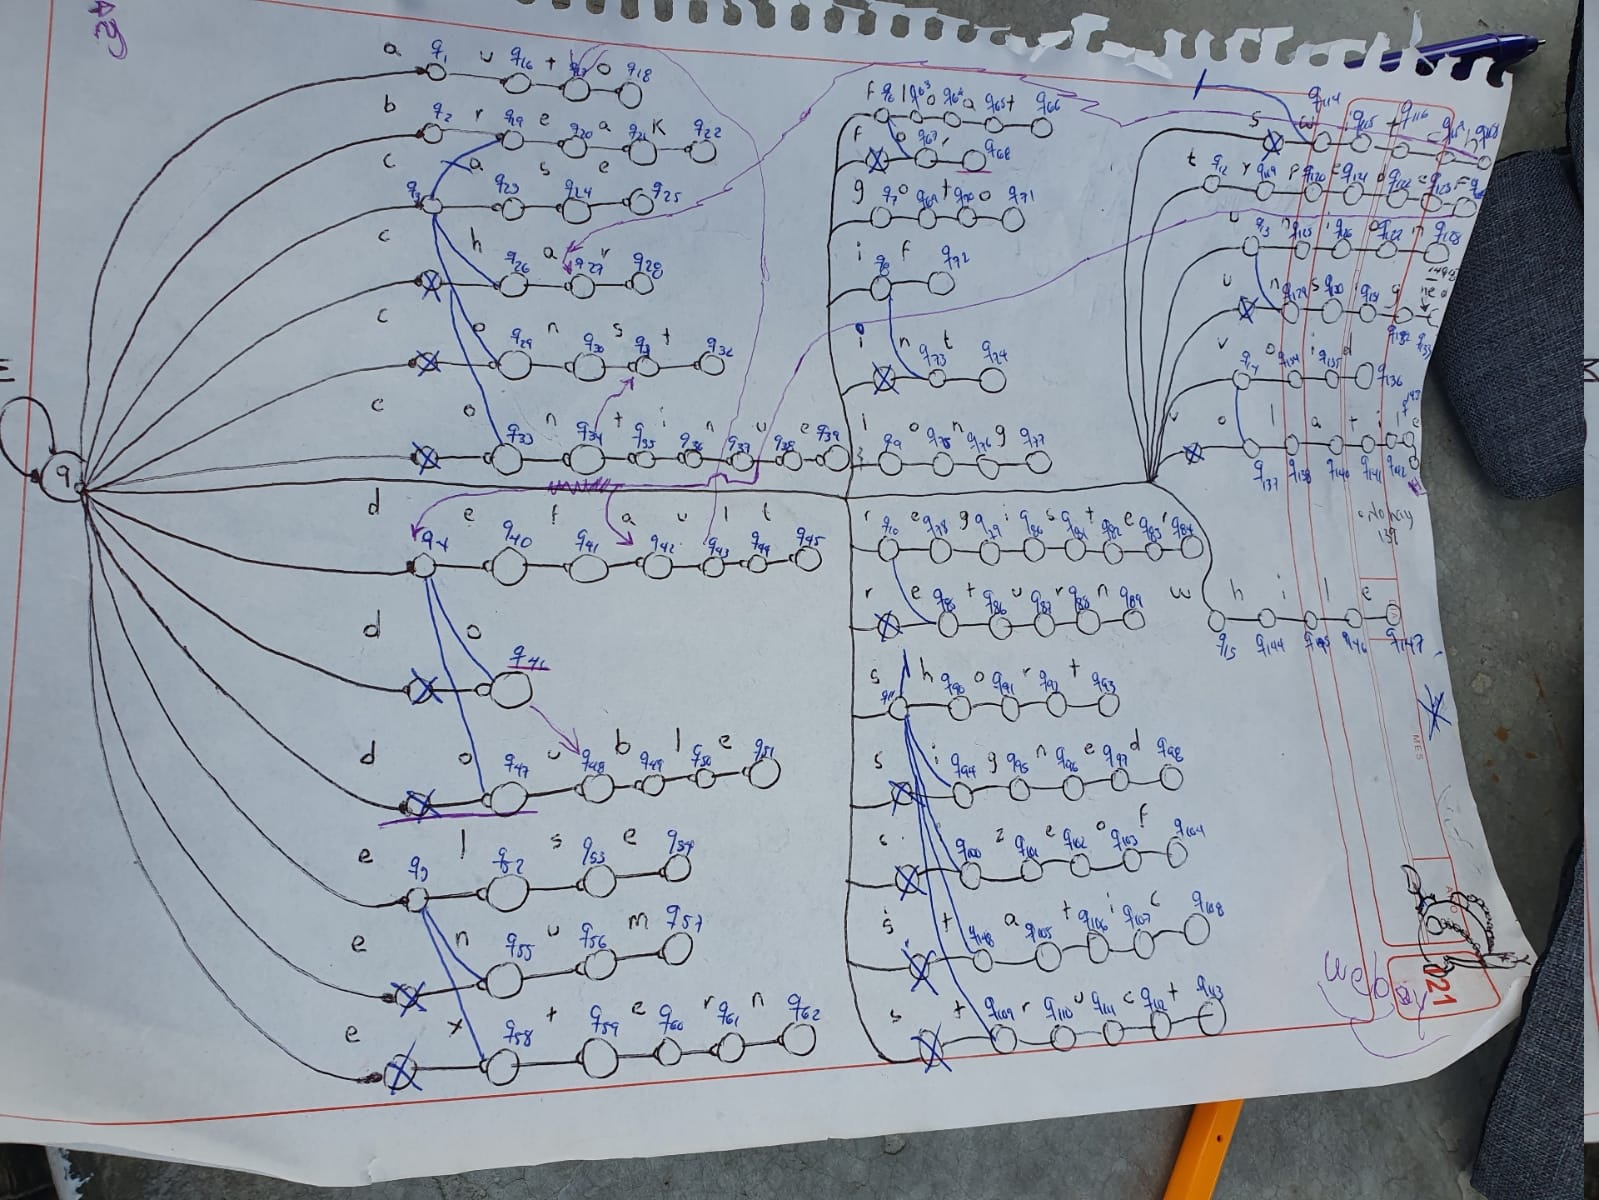
\includegraphics[width=0.8\textwidth]{vabien}
		\caption{Diagrama del autómata no determinista}
	\end{figure}
	
	Posteriormente se realizó la conversión a determinista mediante conjuntos en la tablita como se vio en clase
	
	\begin{figure}[H]
		\centering
		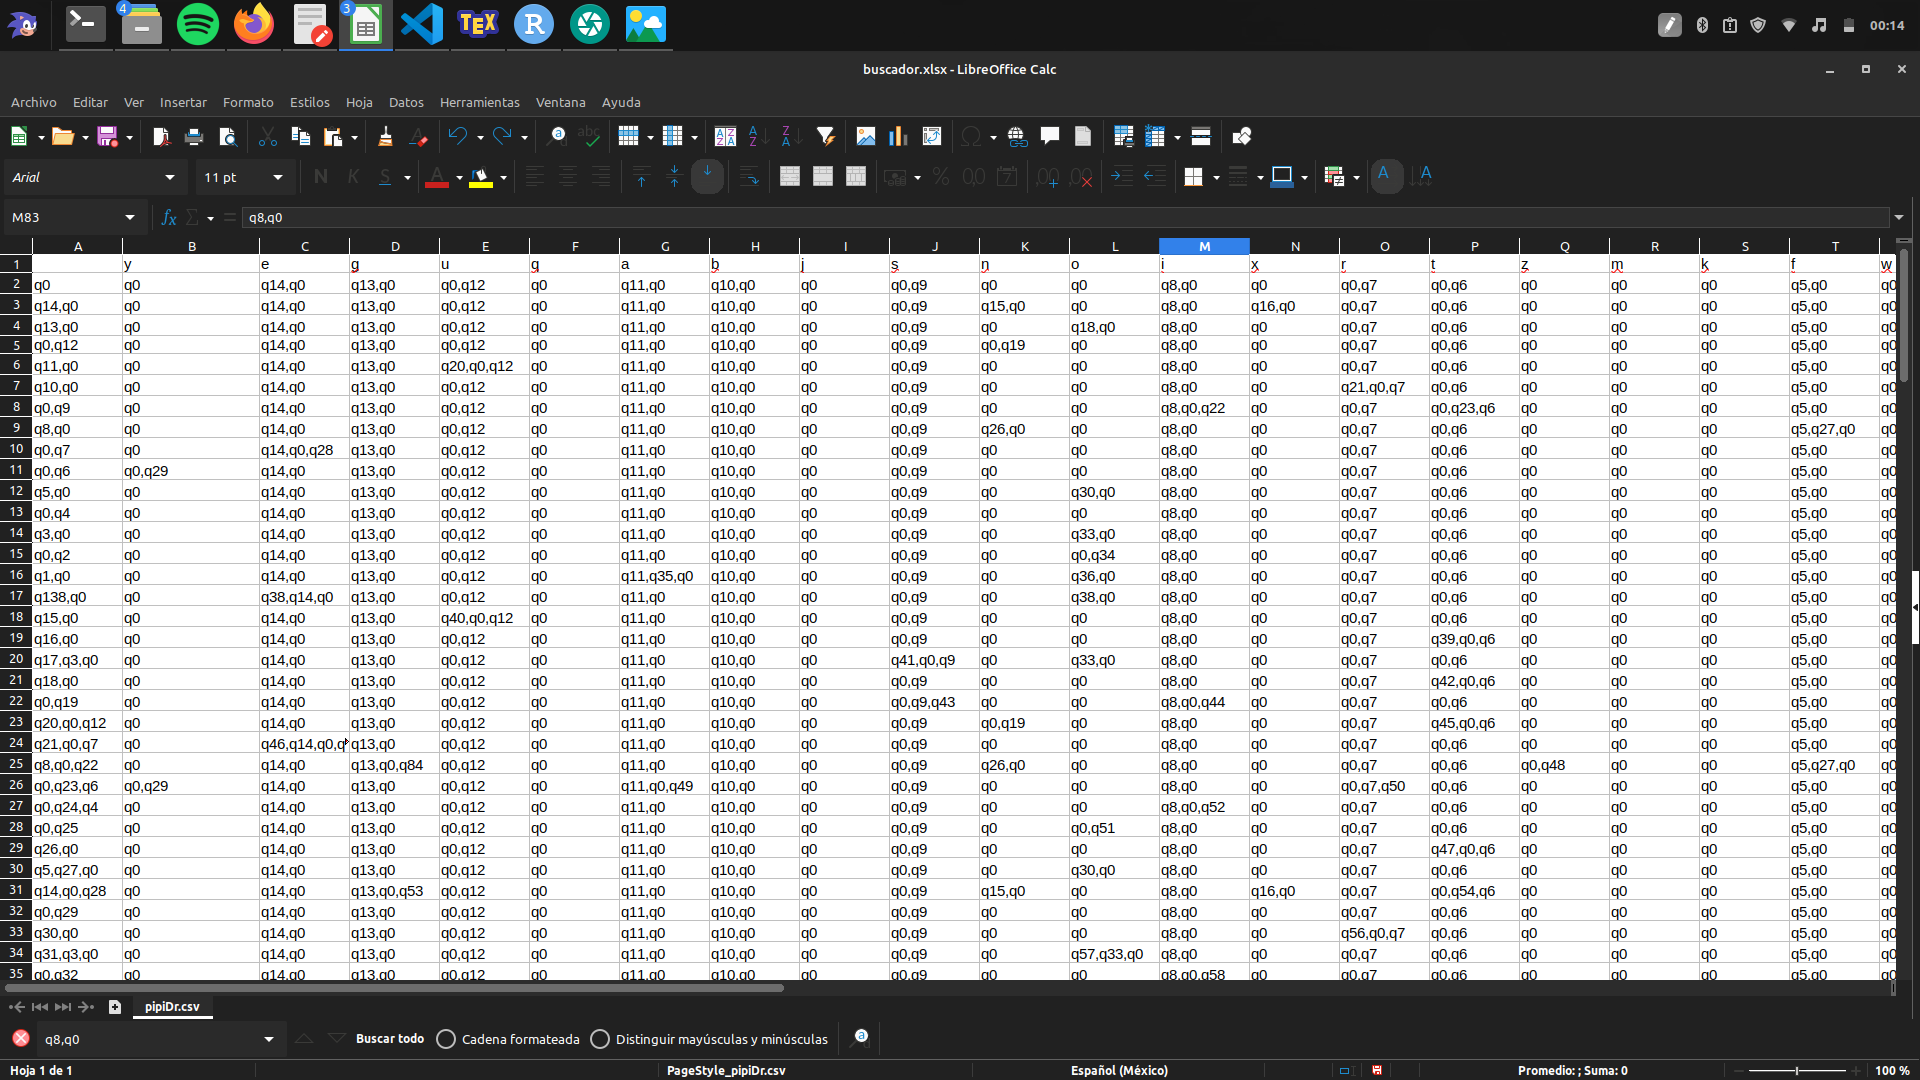
\includegraphics[width=0.8\textwidth]{imagen6}
		\caption{Diagrama del autómata no determinista}
	\end{figure}
	
	\section{Resultados}
	
	
	\begin{figure}[H]
		\centering
		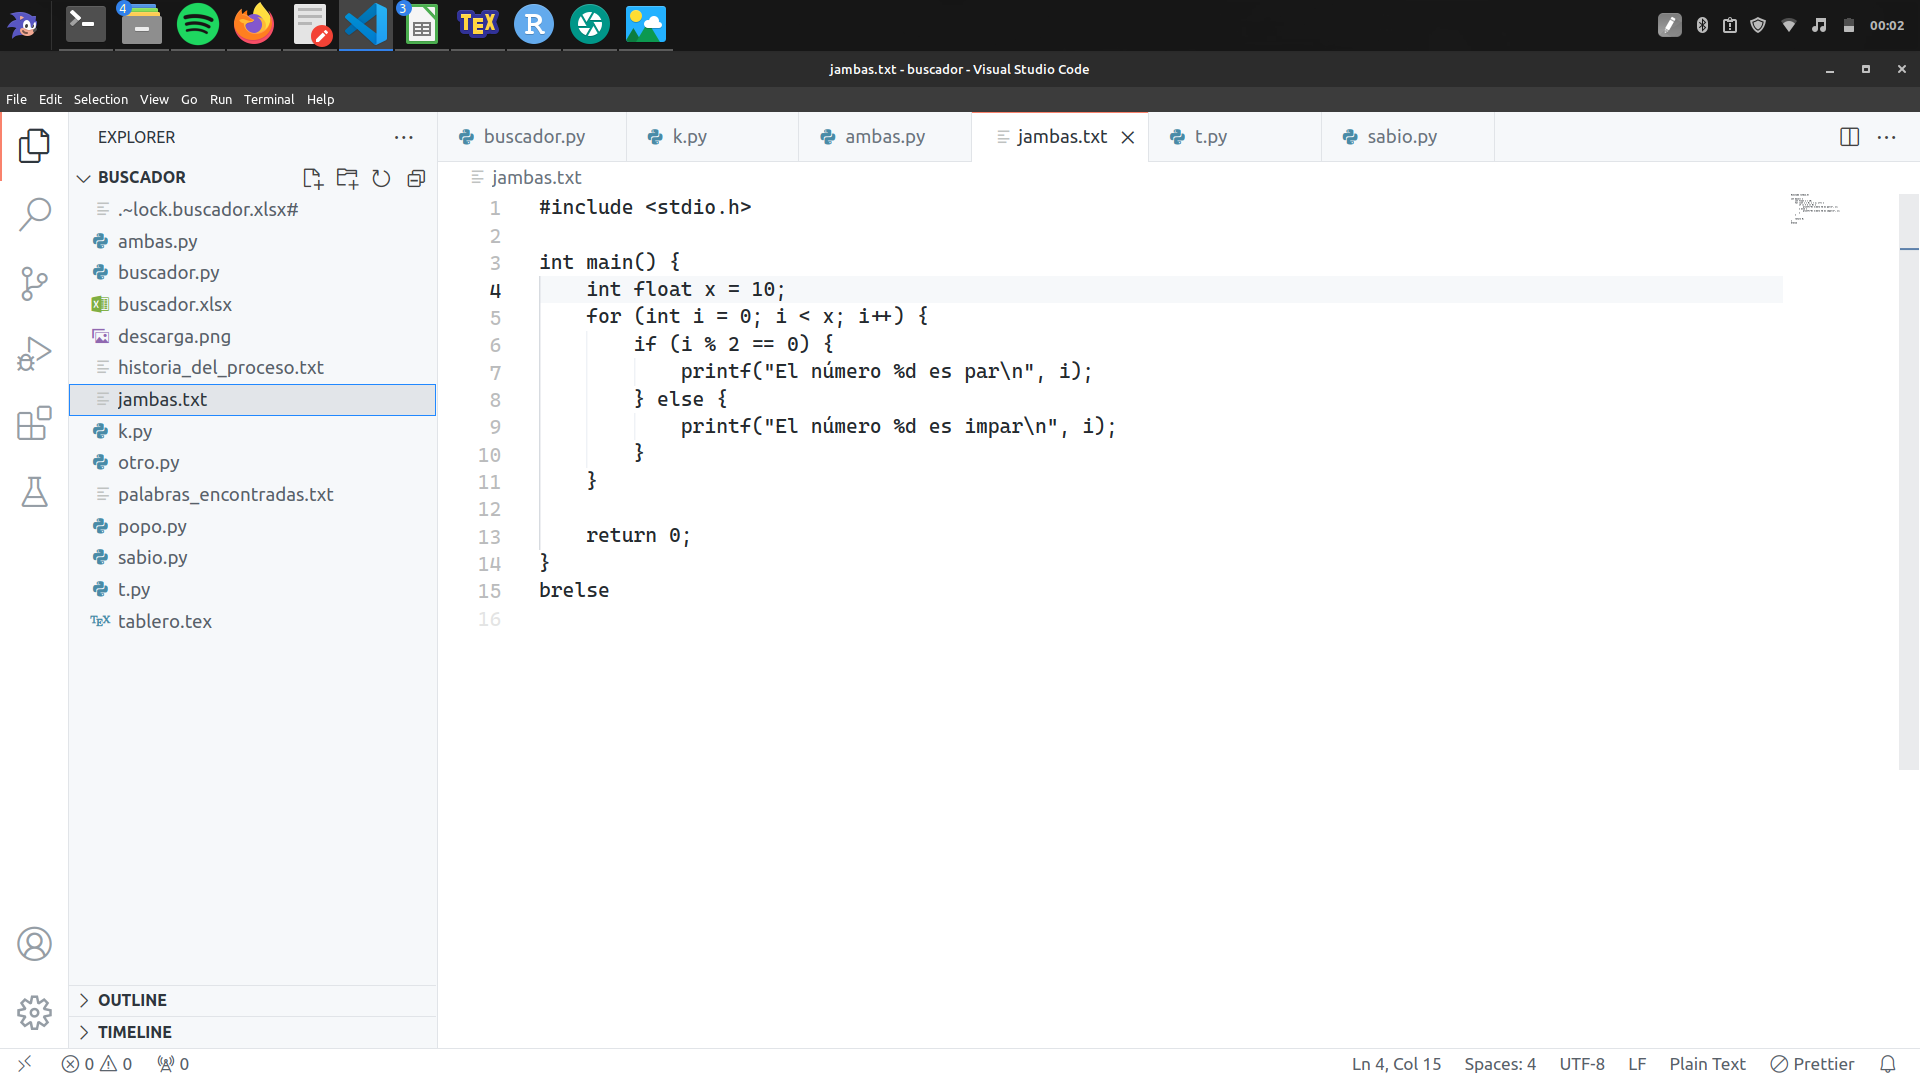
\includegraphics[width=0.8\textwidth]{imagen1.png}
		\caption{Texto a analizar con el autómata}
	\end{figure}
	
	\begin{figure}[H]
		\centering
		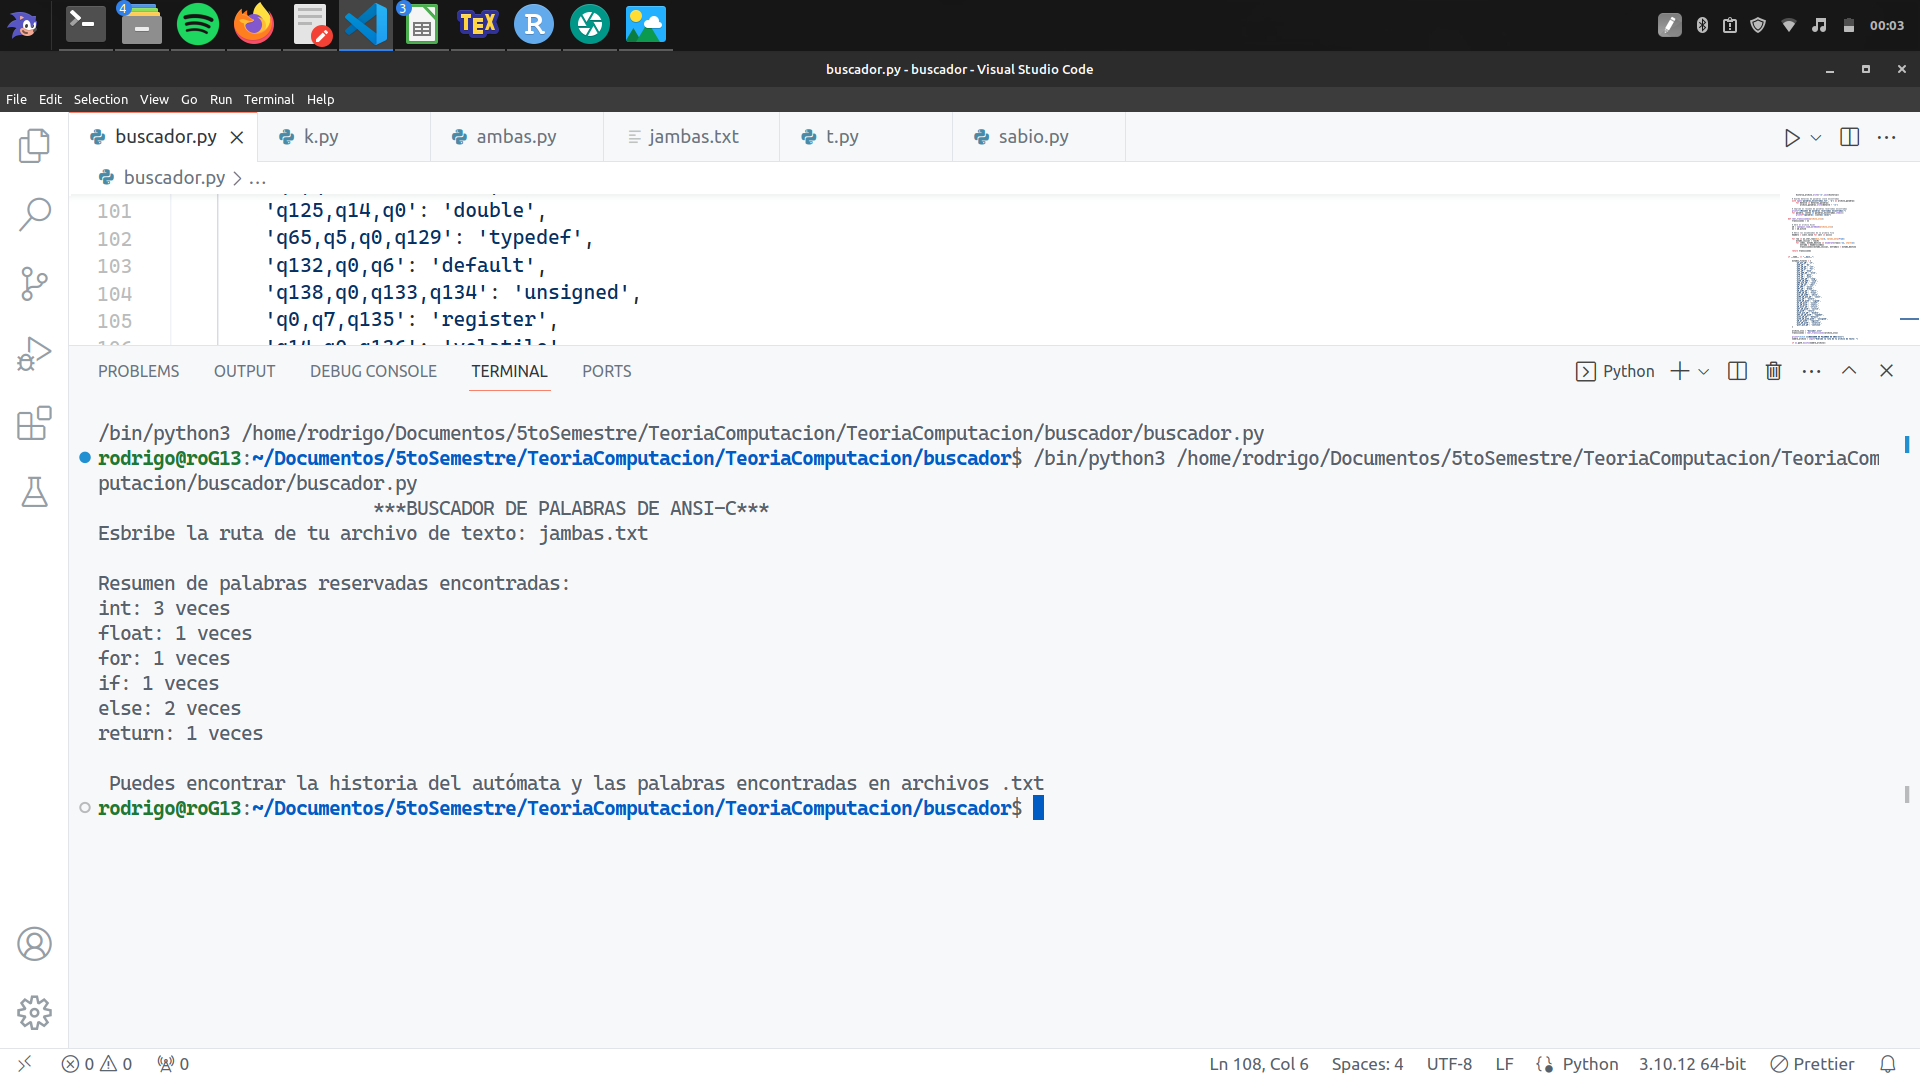
\includegraphics[width=0.8\textwidth]{imagen2.png}
		\caption{Palabras reconocidas}
	\end{figure}
	
	\begin{figure}[H]
		\centering
		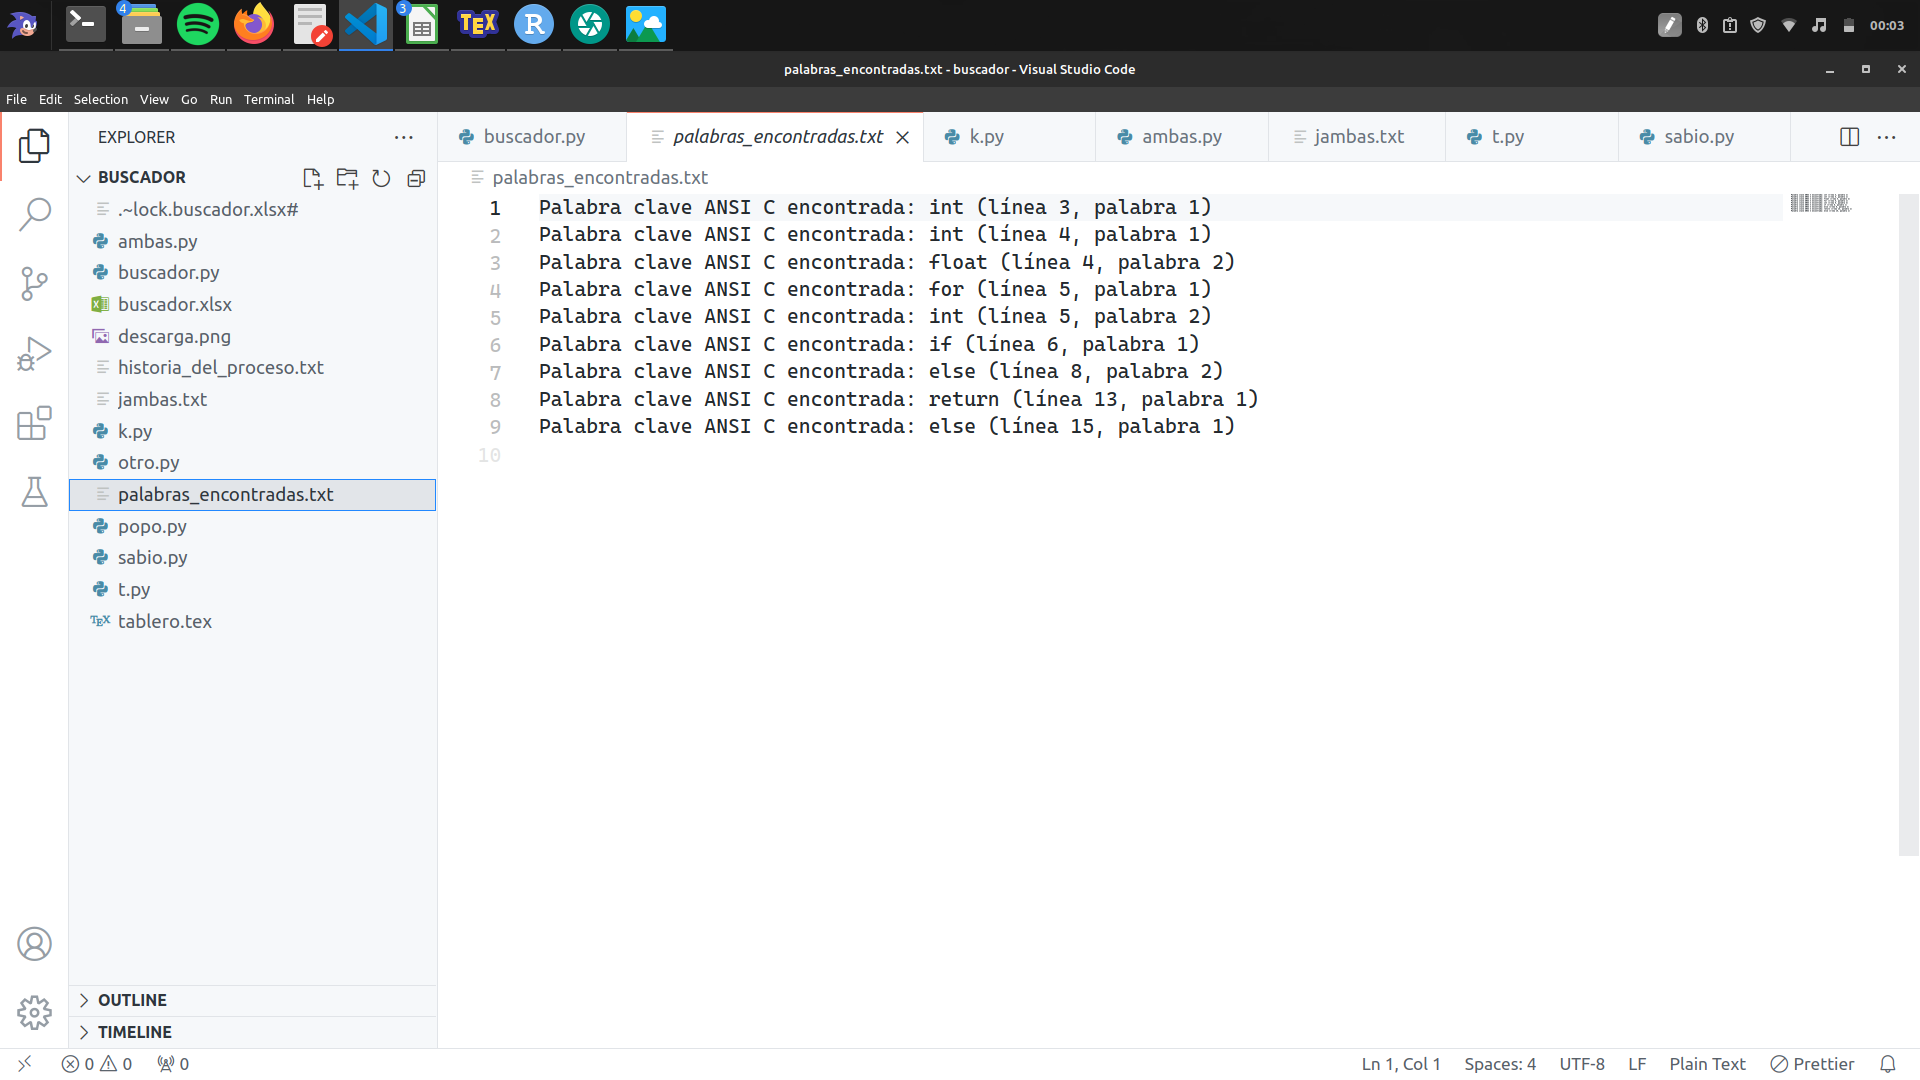
\includegraphics[width=0.8\textwidth]{imagen4.png}
		\caption{Posiciones de las palabras dentro del archivo analizado}
	\end{figure}
	
	\begin{figure}[H]
		\centering
		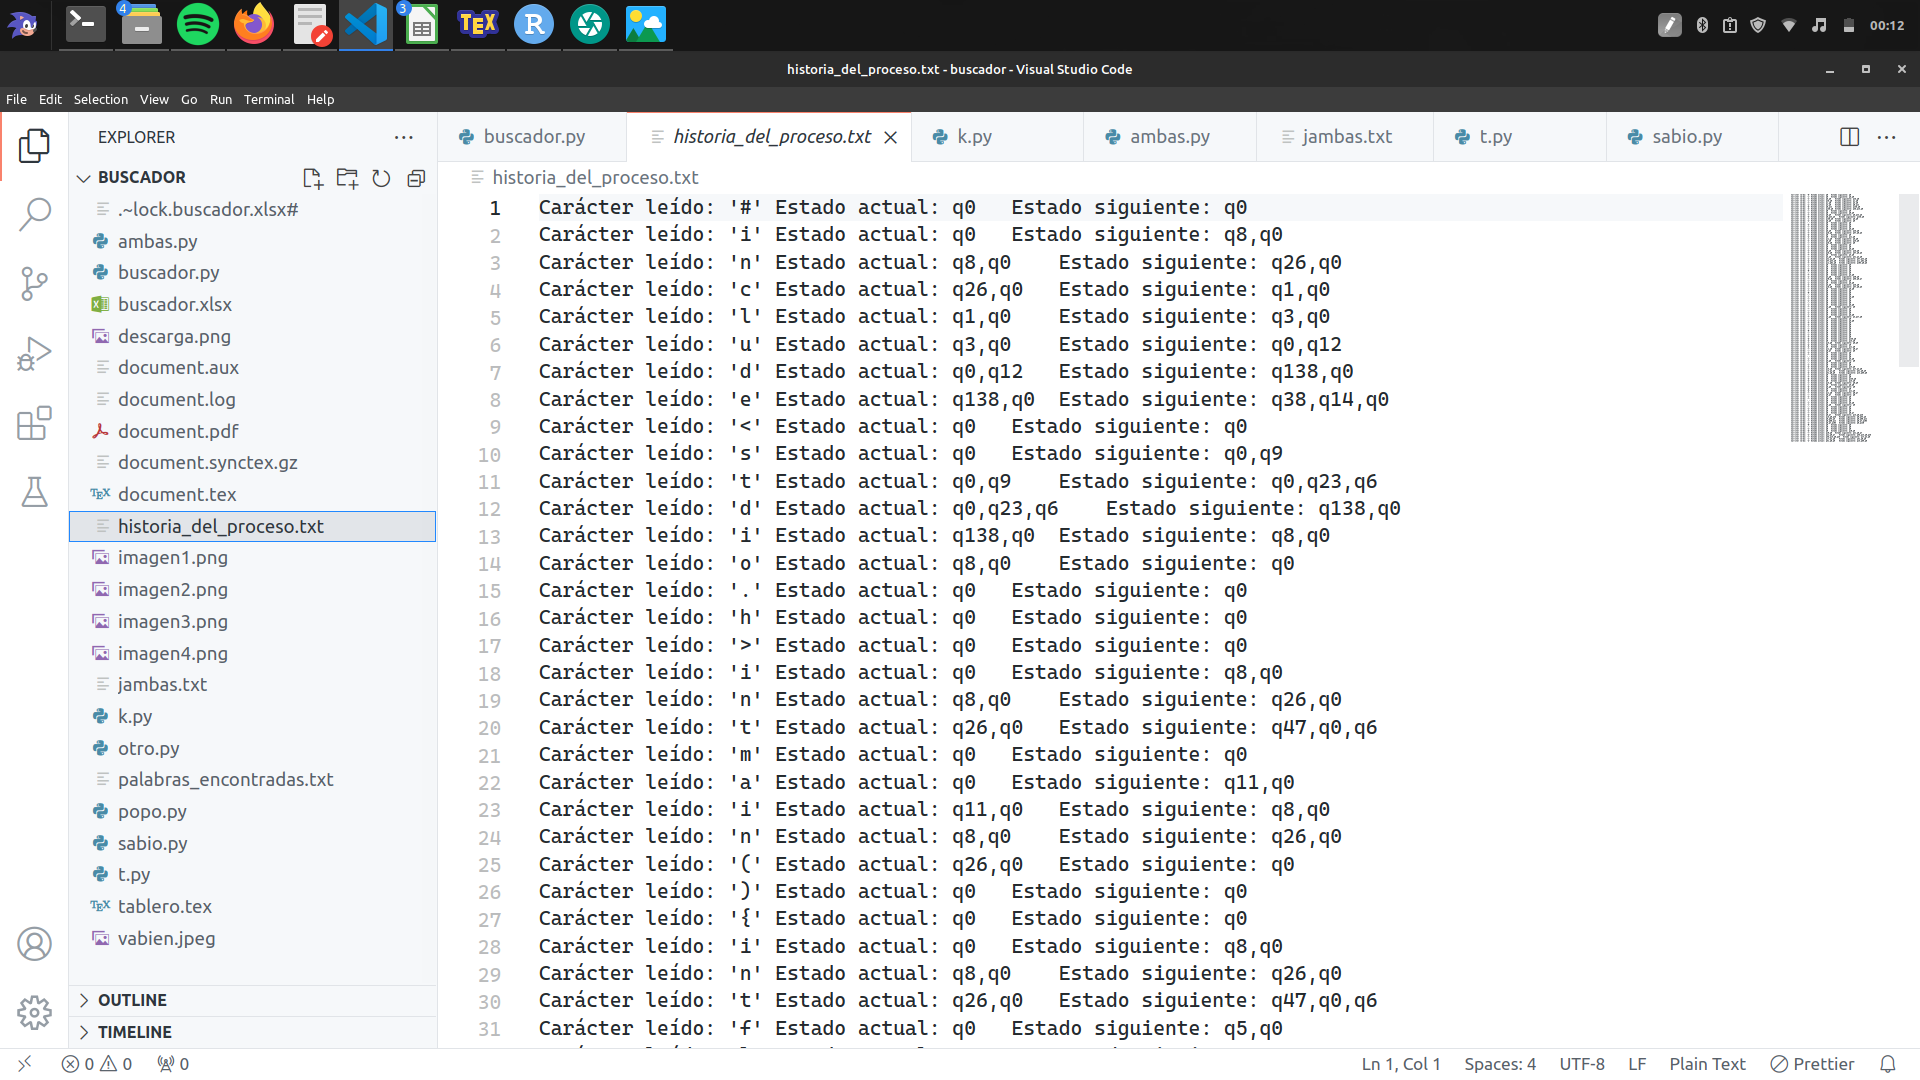
\includegraphics[width=0.8\textwidth]{imagen5}
		\caption{Historia de ejecución}
	\end{figure}
	

	
	
	\section{Código de Implementación}
	
	\begin{lstlisting}
	
	import openpyxl
	import os
	
	def es_palabra_clave(palabra, transiciones):
	estado_actual = 'q0'
	historia_temp = []
	for caracter in palabra:
	# Si el carácter no es alfabético, se reinicia al estado q0
	if not caracter.isalpha():
	historia_temp.append(f"Carácter leído: '{caracter}'\tEstado actual: {estado_actual}\tEstado siguiente: {'q0'}")
	estado_actual = 'q0'
	continue
	
	# Procesa el carácter con las transiciones del DFA
	if (estado_actual, caracter) in transiciones:
	estado_siguiente = transiciones[(estado_actual, caracter)]
	historia_temp.append(f"Carácter leído: '{caracter}'\tEstado actual: {estado_actual}\tEstado siguiente: {estado_siguiente}")
	estado_actual = estado_siguiente
	else:
	return False, [], None
	return estado_actual in estados_finales, historia_temp, estado_actual
	
	def identificar_palabras_clave_en_texto(archivo, transiciones):
	historia = []  # Almacenar la historia del proceso
	palabras_encontradas = {}  # Almacenar palabras reservadas y sus posiciones
	detalles_palabras = []  # Almacenar detalles de las palabras encontradas
	
	with open(archivo, 'r') as archivo_texto:
	for num_linea, linea in enumerate(archivo_texto, start=1):
	palabras = linea.split()
	for num_palabra, palabra in enumerate(palabras, start=1):
	es_clave, historia_temp, estado = es_palabra_clave(palabra, transiciones)
	historia.extend(historia_temp)
	
	if es_clave:
	detalles = f"Palabra clave ANSI C encontrada: {estados_finales[estado]} (línea {num_linea}, palabra {num_palabra})"
	detalles_palabras.append(detalles)
	palabras_encontradas[estados_finales[estado]] = palabras_encontradas.get(estados_finales[estado], 0) + 1
	
	# Guarda la historia del proceso en un archivo
	with open('historia_del_proceso.txt', 'w') as historia_archivo:
	historia_archivo.write('\n'.join(historia))
	
	# Guarda detalles de palabras clave encontradas
	with open('palabras_encontradas.txt', 'w') as archivo_palabras:
	for detalle in detalles_palabras:
	archivo_palabras.write(detalle + '\n')
	
	# Imprime el resumen de palabras reservadas encontradas
	print("\nResumen de palabras reservadas encontradas:")
	for palabra, conteo in palabras_encontradas.items():
	print(f"{palabra}: {conteo} veces")
	
	def leer_transiciones(archivo_xlsx):
	transiciones = {}
	
	# Abre el archivo Excel
	wb = openpyxl.load_workbook(archivo_xlsx)
	ws = wb.active
	
	# Obtén los encabezados de la primera fila
	headers = [cell.value for cell in ws[1]]
	
	for row in ws.iter_rows(min_row=2, values_only=True):
	estado_inicial = row[0]
	for index, estado_destino in enumerate(row[1:-1], start=1):
	entrada = headers[index]
	transiciones[(estado_inicial, entrada)] = estado_destino
	
	return transiciones
	
	
	if __name__ == "__main__":
	
	estados_finales = {
		'q5,q27,q0': 'if',
		'q38,q0': 'do',
		'q47,q0,q6': 'int',
		'q56,q0,q7': 'for',
		'q67,q0': 'enum',
		'q14,q69,q0': 'else',
		'q70,q0': 'goto',
		'q73,q0': 'auto',
		'q13,q85,q0': 'long',
		'q138,q0,q86': 'void',
		'q88,q14,q0': 'case',
		'q91,q0,q7': 'char',
		'q0,q96': 'union',
		'q97,q0': 'break',
		'q0,q102,q6': 'short',
		'q105,q0,q6': 'float',
		'q14,q0,q106': 'while',
		'q108,q0,q23,q6': 'const',
		'q112,q0': 'extern',
		'q138,q0,q133': 'signed',
		'q5,q0,q115': 'sizeof',
		'q1,q0,q116': 'static',
		'q0,q117,q6': 'struct',
		'q37,q0,q118': 'switch',
		'q0,q120': 'return',
		'q125,q14,q0': 'double',
		'q65,q5,q0,q129': 'typedef',
		'q132,q0,q6': 'default',
		'q138,q0,q133,q134': 'unsigned',
		'q0,q7,q135': 'register',
		'q14,q0,q136': 'volatile',
		'q137,q14,q0': 'continue'
	}
	
	archivo_xlsx = "buscador.xlsx"
	transiciones = leer_transiciones(archivo_xlsx)
	
	print("\t\t\t ***BUSCADOR DE PALABRAS DE ANSI-C***")
	nombre_archivo = input("Esbribe la ruta de tu archivo de texto: ")
	
	if os.path.exists(nombre_archivo):
	identificar_palabras_clave_en_texto('jambas.txt', transiciones)
	print("\n Puedes encontrar la historia del autómata y las palabras encontradas en archivos .txt")
	
	else:
	print(f"El archivo {nombre_archivo} no existe.")
	
	
	\end{lstlisting}

	
	
\end{document}